\subsection{\software{Netabc}: a computer program for estimation of contact
network parameters with kernel-assisted ABC}

\software{Netabc} is a computer program to perform statistical inference of
contact network parameters from an estimated transmission tree using
kernel-assisted \gls{ABC}. The program combines three major components: Gillespie
simulation, to simulate transmission trees on contact networks; the tree
kernel, to compare transmission trees; and adaptive \gls{ABC}-\gls{SMC}, to
maintain a population of particles and advance it toward the \gls{ABC} target
distribution. We give a high-level overview of the program here, before
describing these three components in detail. \software{Netabc} takes as input
an estimated transmission tree, which can be derived from a viral phylogeny by
rooting and time-scaling as described in \cref{subsec:phylodynamics} or
estimated by other methods~\autocite{cottam2008integrating,
jombart2011reconstructing, ypma2012unravelling, morelli2012bayesian,
didelot2014bayesian}. We variously refer to this estimated transmission tree as
the observed tree, input tree, or true tree.

As described in \cref{sec:smc}, \software{netabc} keeps track of a population
of particles $x^{(k)}$, each of which contains particular parameter values
$\theta^{(k)}$ for the model we are trying to fit. A small number of contact
networks $z^{(k)}$ are generated for each particle, in accordance with that
particle's parameters. An epidemic is simulated over each of these networks
using Gillespie simulation, and by keeping track of its progress, a
transmission tree is obtained. Thus, each particle becomes associated with
several simulated transmission trees. These trees are compared to the input
tree using the tree kernel. Particles are weighted according to the similarity
of their associated simulated trees with the true tree, with more similar trees
receiving higher weights. The particles are iteratively perturbed to explore
the parameter space, and particles with simulated trees too distant from the
true tree are periodically dropped and resampled. Once a convergence criterion
is attained, the final set of particles is used as a Monte Carlo approximation
to the target distribution of \gls{ABC}, which is assumed to resemble the
posterior distribution on model parameters (see \cref{sec:abc}). A graphical
schematic of this algorithm is given in \cref{fig:abcsmc}.

\begin{figure}
    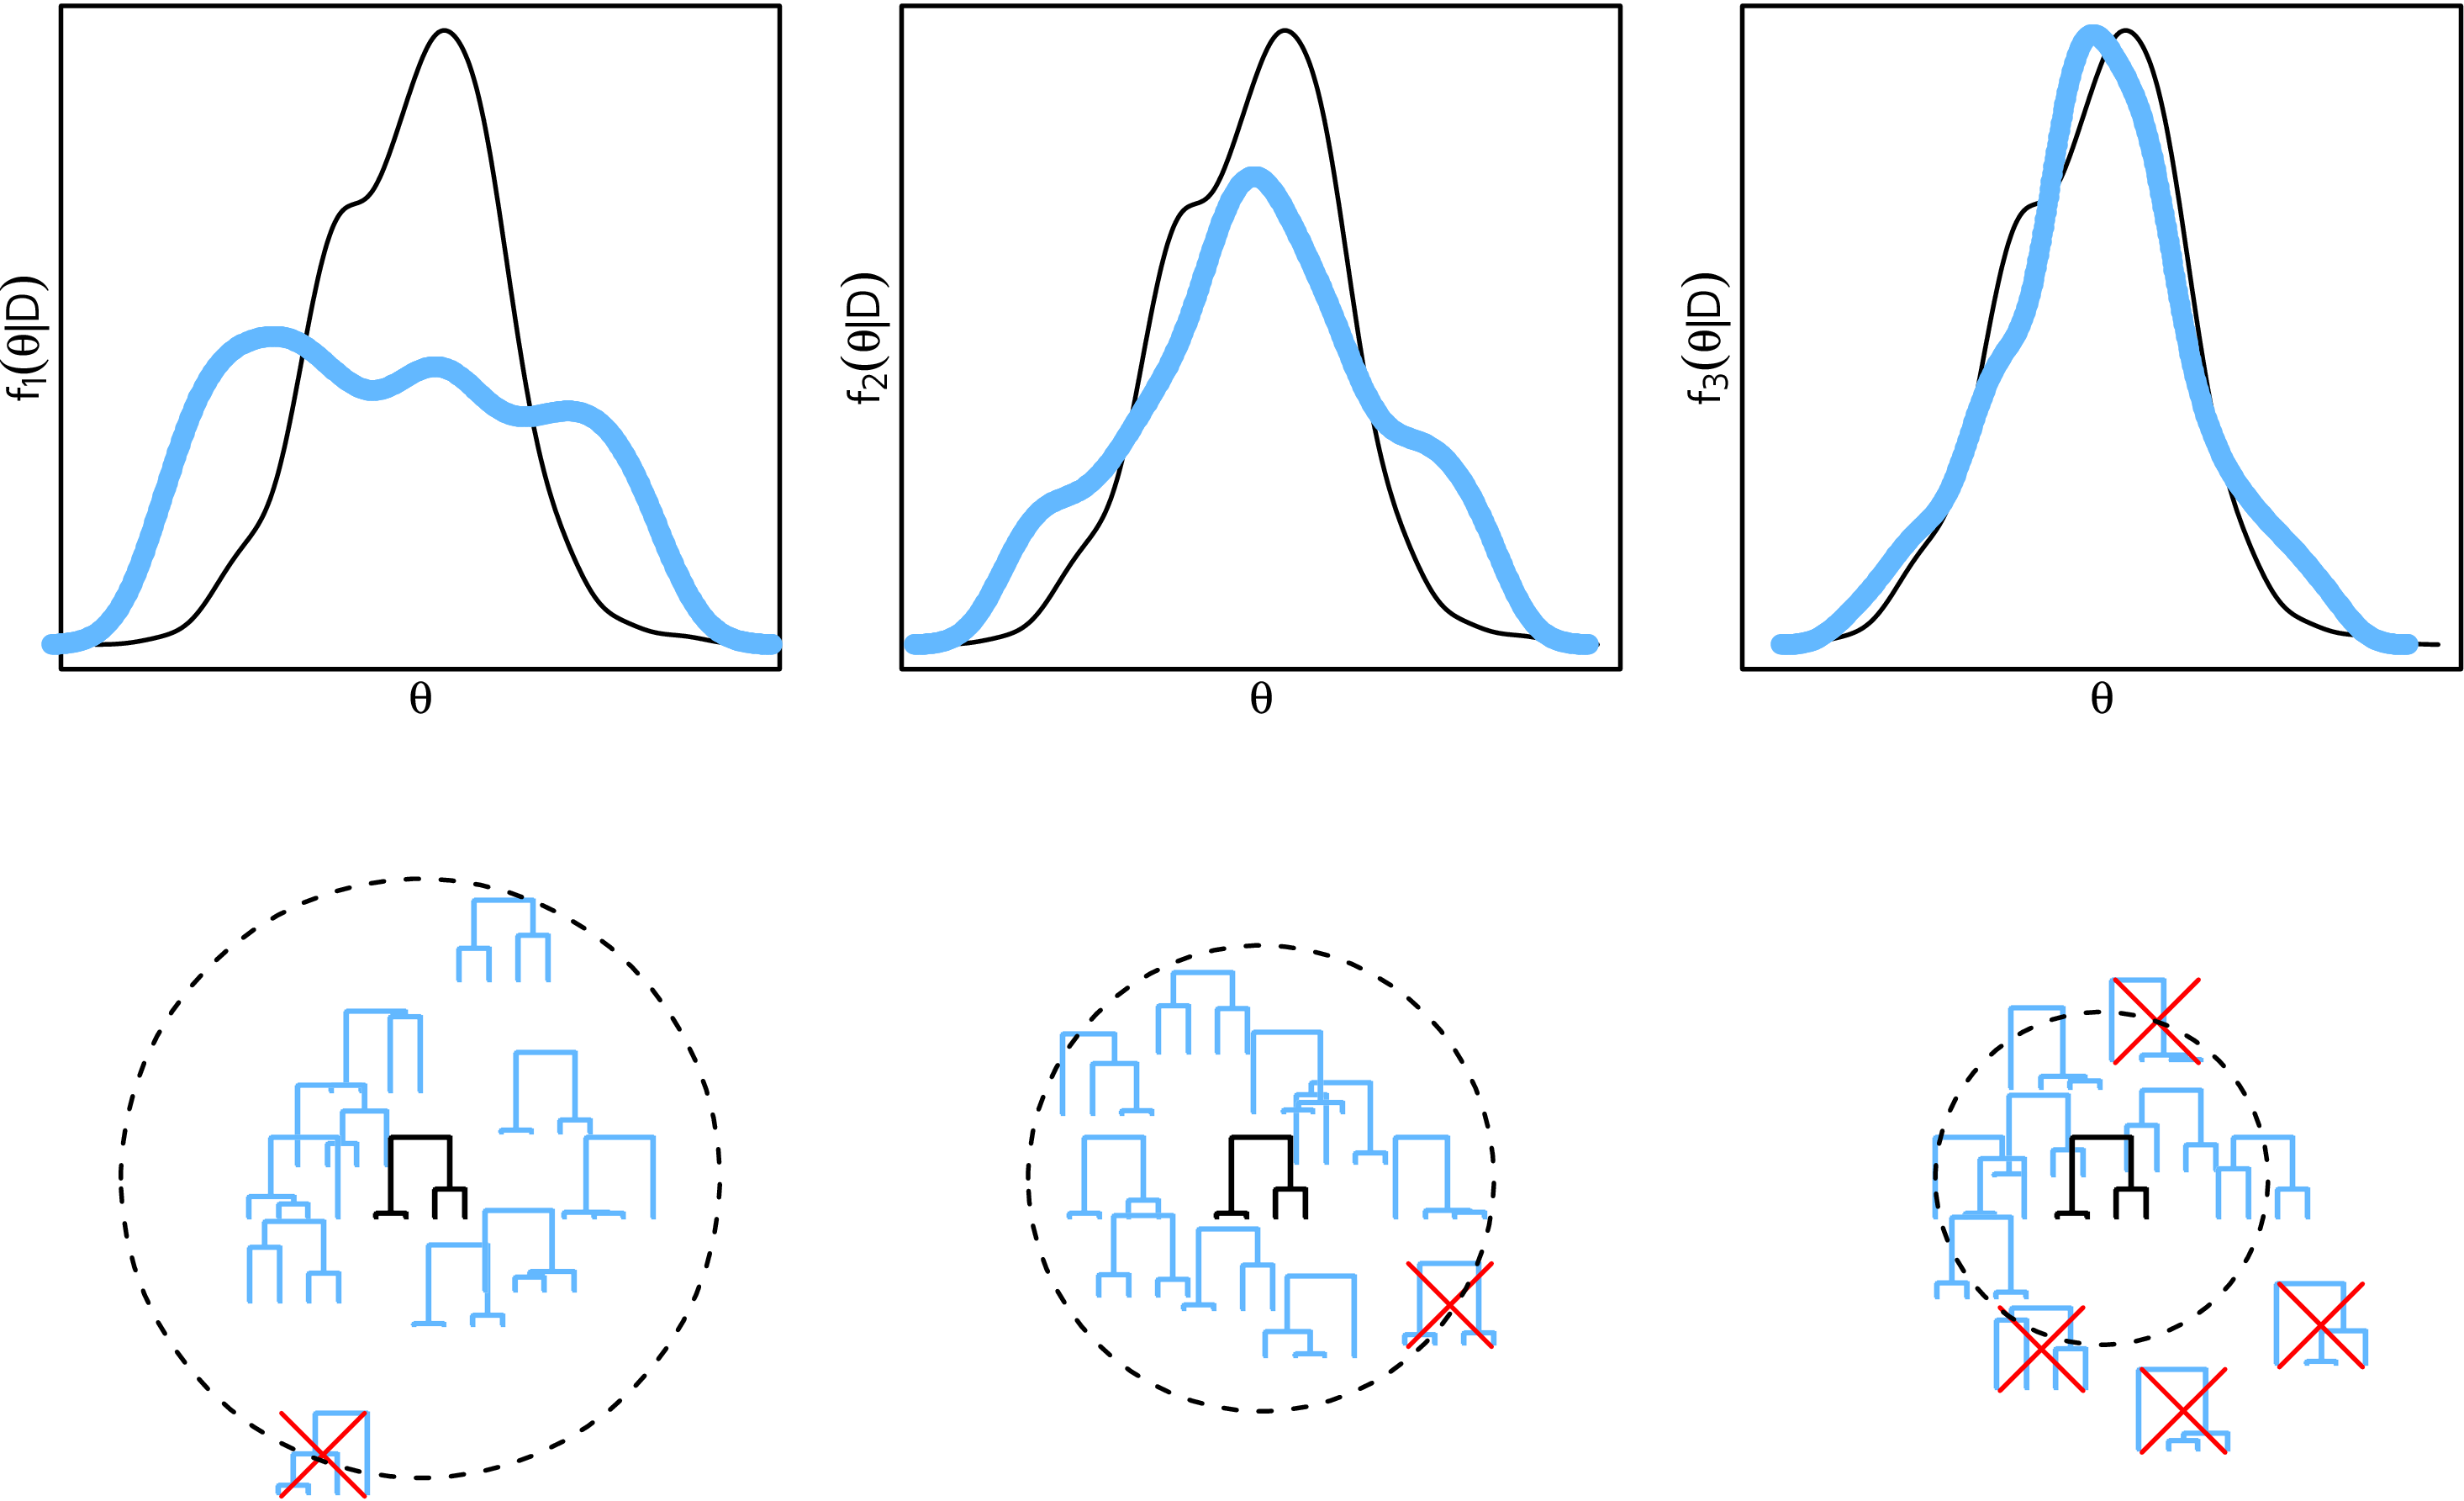
\includegraphics{abc-smc.pdf}
    \caption[Graphical schematic of the ABC-SMC algorithm implemented in \software{netabc}.]{
      Graphical schematic of the \gls{ABC}-\gls{SMC} algorithm implemented in
      \software{netabc}. Particles are initially drawn from their prior
      distributions, making the initial population a Monte Carlo approximation
      to the prior. At each iteration, particles are perturbed, and a distance
      threshold around the true tree contracts. Particles are rejected, and
      eventually resampled, when all their associated simulated trees lie
      outside the threshold. As the algorithm progresses, the population
      smoothly approaches a Monte Carlo approximation of the \gls{ABC} target
      distribution, which is assumed to resemble the posterior.
    }
    \label{fig:abcsmc}
\end{figure}

\software{Netabc} is written in the \software{C} programming language. The
\software{igraph} library~\autocite{csardi2006igraph} is used to generate and
store contact networks and phylogenies. Judy arrays~\autocite{baskins2004judy}
are used for hash tables and dynamic programming matrices. The
\gls{GSL}~\autocite{gough2009gnu} is used to generate random draws from
probability distributions, and to perform the bisection step in the adaptive
\gls{ABC}-\gls{SMC} algorithm. Parallelization is implemented with POSIX
threads~\autocite{barney2009posix}. In addition to the \software{netabc} binary
to perform kernel-assisted \gls{ABC}, we provide three additional stand-alone
utilities: \software{treekernel}, to calculate the tree kernel;
\software{nettree}, to simulate a transmission tree over a contact network; and
\software{treestat}, to compute various summary statistics of phylogenies. The
programs are freely available at \url{https://github.com/rmcclosk/netabc}.

To check that our implementation of Gillespie simulation was correct, we
reproduced Figure 1A of \textcite{leventhal2012inferring} (our
\cref{fig:leventhal}), which plots the unbalancedness of transmission trees
simulated over four network models at various levels of pathogen
transmissibility. Our implementation of adaptive ABC-SMC was tested by applying
it to the same mixture of Gaussians used by \citeauthor{del2012adaptive} to
demonstrate their method (originally used by~\textcite{sisson2007sequential}).
We were able to obtain a close approximation to the function (see
\cref{fig:smctest}), and attained the stopping condition used by the authors in
a comparable number of steps. To check that the algorithm would converge to a
bimodal distribution, we also applied it to a mixture of two Gaussians with
means $\pm$4 and variances 1. The algorithm was able to recover both peaks
(\cref{fig:smctest2}).

\subsubsection*{Epidemic simulation}
\label{subsubsec:nettree}

The simulation of epidemics, and the corresponding transmission trees, over
contact networks is performed in \software{netabc} using the Gillespie
simulation algorithm~\autocite{gillespie1976general}. This method has been
independently implemented and applied by several
authors~\autocite[\textit{e.g.}][]{o2011contact, robinson2013dynamics,
leventhal2012inferring, groendyke2011bayesian, villandre2016assessment}.
\textcite{groendyke2011bayesian} published their implementation as an
\software{R} package, but since the \gls{SMC} algorithm is quite
computationally intensive, we chose to implement our own version in
\software{C}.

Let $G = (V, E)$ be a directed contact network. We assume the individual nodes
and edges of $G$ follow the dynamics of the \gls{SIR}
model~\autocite{kermack1927contribution}. Each directed edge $e = (u, v)$ in
the network is associated with a transmission rate $\beta_e$, which indicates
that, once $u$ becomes infected, the waiting time until $u$ infects $v$ is
distributed as $\Exponential(\beta_e)$. Note that $v$ may become infected
before this time has elapsed, if $v$ has other incoming edges. $v$ also has a
removal rate $\gamma_v$, so that the waiting time until removal of $v$ from the
population is $\Exponential(\gamma_v)$. Removal may correspond to death or
recovery with immunity, or a combination of both, but in our implementation
recovered nodes never re-enter the susceptible population. We define a
\defn{discordant edge} as an edge $(u, v)$ where $u$ is infected and $v$ has
never been infected.

To describe the algorithm, we introduce some notation and variables. Let
$\inc(v)$ be the set of incoming edges to $v$, and $\out(v)$ be the set of
outgoing edges from $v$. Let $I$ be the set of infected nodes in the network,
$R$ be the set of removed nodes, and $S$ be the remaining susceptible nodes,
and $D$ be the set of discordant edges in the network. Let $\beta$ be the total
transmission rate over all discordant edges, and $\gamma$ be the total removal
rate of all infected nodes,
\[
  \beta = \sum_{e \in D} \beta_e, \quad
  \gamma = \sum_{v \in I} \gamma_v.
\]
The variables $S$, $I$, $R$, $D$, $\beta$, and $\gamma$ are all updated as the
simulation progresses. When a node $v$ becomes infected, it is deleted from $S$
and added to $I$. Any formerly discordant edges in $\inc(v)$ are deleted from
$D$, and edges in $\out(v)$ to nodes in $S$ are added to $D$. If $v$ is later
removed, it is deleted from $I$ and added to $R$, and any discordant edges in
$\out(v)$ are deleted from $D$. At the time of either infection or removal, the
variables $\beta$ and $\gamma$ are updated to reflect the changes in the
network. Since these updates are straightforward, we do not write them
explicitly in the algorithm.

\newcommand{\tip}{\mathit{tip}}

The Gillespie simulation algorithm is given as Algorithm~\ref{alg:nettree}. The
transmission tree $T$ is simulated along with the epidemic. We keep a map
called $\tip$, which maps infected nodes in $I$ to the tips of $T$. The
simulation continues until either there are no discordant edges left in the
network, or we reach a user-defined cutoff of time ($t_{\max}$) or number of
infections ($I_{\max}$). We use the notation $\Uniform(0, 1)$ to indicate a
number drawn from a uniform distribution on $(0, 1)$, and likewise for
$\Exponential(\lambda)$. The combined number of internal nodes and tips in $T$
is denoted $|T|$.

\begin{algorithm}
  \label{alg:nettree}
  \caption{Simulation of an epidemic and transmission tree over a contact network}
  \begin{algorithmic}
    \State infect a node $v$ at random, updating $S$, $I$, $D$, $\beta$ and $\gamma$
    \State $T \gets$ a single node with label $1$
    \State $\tip[v] \gets 1$
    \State $t \gets 0$
    \While{$D \neq \emptyset$ and $|I| + |R| < I_{\max}$ and $t < t_{\max}$}
      \State $s \gets \min(t_{\max} - t, \Exponential(\beta + \gamma))$
      \For{$v \in \tip$}
        \State{extend the branch length of $\tip[v]$ by $s$}
      \EndFor
      \State $t \gets t + s$
      \If{$t < t_{\max}$}
        \If{$\Uniform(0, \beta + \gamma) < \beta$}
          \State choose an edge $e = (u, v)$ from $D$ with probability $\beta_e / \beta$
                 and infect $v$
          \State add tips with labels $(|T|+1)$ and $(|T|+2)$ to $T$
          \State connect the new nodes to $\tip[v]$ in $T$, with branch lengths $0$
          \State $\tip[v] \gets |T|-1$
          \State $\tip[u] \gets |T|$
        \Else
          \State choose a node $v$ from $I$ with probability $\gamma_v / \gamma$
                 and remove $v$
          \State delete $v$ from $\tip$
        \EndIf
        \State update $S$, $I$, $R$, $D$, $\beta$, and $\gamma$
      \EndIf
    \EndWhile
  \end{algorithmic}
\end{algorithm}

\subsubsection{Phylogenetic kernel}

The tree kernel developed by \textcite{poon2013mapping} provides a
comprehensive similarity score between two phylogenetic trees, via the
dot-product of the two trees' feature vectors in the infinite-dimensional space
of all possible subset trees with branch lengths (see \cref{subsec:treeshape}).
The kernel was implemented using the fast algorithm developed by
\textcite{moschitti2006making}. First, the production rule of each node, which
is the total number of children and the number of leaf children, is recorded.
The nodes of both trees are ordered by production rule, and a list of pairs of
nodes sharing the same production rule is created. These are the nodes for
which the value of the tree kernel must be computed - all other pairs have a
value of zero. The pairs to be compared are then re-ordered so that the child
nodes are always evaluated before their parents. Due to its recursive
definition, ordering the pairs in this way allows the tree kernel to be
computed by dynamic programming. The complexity of this implementation is
$O(|T_1||T_2|)$, where $|T|$ counts the number of nodes in the tree $T$.

The tree kernel cannot be used directly as a distance measure for \gls{ABC},
since it is maximized, not minimized, when the two trees being compared are the
same. Therefore, we defined the distance between two trees as
\[
  \rho(T_1, T_2) = 1 - \frac{K(T_1, T_2)}{\sqrt{K(T_1, T_1) K(T_2, T_2)}},
\]
which is a number between 0 and 1 minimized when $T_1 = T_2$. This is similar
to the normalization used by \textcite{collins2002new, poon2013mapping}.

\subsubsection*{Adaptive sequential Monte Carlo for Approximate Bayesian computation}
\label{subsubsec:adaptsmc}

We implemented the adaptive \gls{SMC} algorithm for \gls{ABC} developed by
\textcite{del2012adaptive}. This algorithm is similar to the reference
\gls{ABC}-\gls{SMC} algorithm described in \cref{subsec:abcalg}, except that
the sequence of tolerances $\varepsilon_i$ is automatically determined rather
than specified in advance. The tolerances are chosen such that the \gls{ESS} of
the particle population, which indicates the quality of the Monte Carlo
approximation (see \cref{subsec:sis}), decays at a controlled rate. A
sudden precipitous drop in \gls{ESS} would indicate that only a small number of
particles had non-zero importance weights, which would result in a very poor
Monte Carlo approximation to the target distribution. This situation is
referred to as the ``collapse'' of the approximation, and is mitigated by the
adaptive approach. A single parameter $\alpha$ (not to be confused with the
\gls{BA} model parameter) controls the decay rate, with $\varepsilon_i$ being
chosen to satisfy
\[
  \ESS(w_i) = \alpha \ESS(w_{i-1}).
\]
Here, $w_i$ is the vector of weights at the $i$th step. Note that, since $w_i$
depends on $\varepsilon_i$, this equation solves for the updated weights and
the updated tolerance simultaneously. As pointed out by
\textcite{del2012adaptive}, the equation has no analytic solution, but can be
solved numerically by bisection. The forward kernels $K_i$ are taken to be
\gls{MCMC} kernels with stationary distributions $\pi_{\varepsilon_i}$ and
proposal distributions
\[
  q_i(\theta, \theta') \prod_{k=1}^M \Pr(z_i^{(k)'} \mid \theta'),
\]
where $\theta$ is the vector of model parameters and $z_k$ are $M$ datasets
simulated according to $\theta'$. In our implementation, $q$ is either a
Gaussian proposal for continuous parameters, or a Poisson proposal for discrete
parameters. For the Poisson proposals, the number of steps to move the particle
is drawn from a Poisson distribution, and the direction in which to move the
particle is chosen uniformly at random. For both proposals, the variance was
set equal to twice the empirical variance of the particles,
following~\autocite{beaumont2009adaptive, del2012adaptive}. The backwards
kernels are
\[
  L_{i-1}(x', x) = \frac{\pi_n(x)K(x, x')}{\pi_n(x')}.
\]
When substituted into \cref{eq:smcwt}, the forward kernels $K(x, x')$ and
densities $\pi_n(x') = \pi_{\varepsilon_n}(x')$ cancel out, and we are left
with the weight update 
\begin{align*}
  w_i(x) 
    &\propto w_{i-1}(x) \frac{\pi_n(x \mid y)}{\pi_{i-1}(x \mid y)} \\
    &= w_{i-1}(x) \frac{\pi(x) \pi_i(y \mid x)}{\pi(x) \pi_{i-1}(y \mid x)} \\
    &= w_{i-1}(x) \frac{\sum_{k=i}^M \I_{A_{\varepsilon_i, y}}(z_k)}
            {\sum_{k=i}^M \I_{A_{\varepsilon_{i-1}, y}}(z_k)}.
\end{align*}
In other words, when the distance threshold $\varepsilon_{i-1}$ is contracted
to $\varepsilon_i$, the particles' weights are multiplied by the proportion of
simulated datasets which are still inside the new threshold. The algorithm may
be stopped when one of two termination conditions is reached. The user may
specify a final tolerance $\varepsilon$, or a final acceptance rate of the
\gls{MCMC} kernel. The latter condition stops the algorithm when the particles
are not moving around very much, implying little change in the estimated
target.

\subsection{Analysis of \acrlong{BA} model}

We investigated four parameters related to the \gls{BA} model, denoted
\gls{N}, \gls{m}, \gls{alpha}, \gls{I}. The first three of these are parameters
of the model itself, while \gls{I} is related to the simulation of transmission
trees over the network. However, we will refer to all four as \gls{BA}
parameters. \gls{N} denotes the total number of nodes in the network, or
equivalently, susceptible individuals in the population. When a node is added
to the network, \gls{m} new undirected edges are added incident to it, and are
attached to existing nodes of degree $k$ with probability proportional to
$k^\alpha + 1$ (\cref{subsec:pa}). To simulate transmission trees over a
\gls{BA} network, we allowed an epidemic to spread until \gls{I} nodes were
infected, and sampled a transmission tree at that time. The \gls{alpha}
parameter is unitless, while \gls{m} has units of edges or connections per
vertex, and \gls{N} and \gls{I} both have units of nodes or individuals.

We assumed that all contacts had symmetric transmission risk, which was
implemented by replacing each undirected edge in the network with two directed
edges (one in each direction). Nodes in our networks followed simple \gls{SI}
dynamics, meaning that they became infected at a rate proportional to their
number of infected neighbours, and never recovered. We did not consider the
time scale of the transmission trees in these simulations, only their shape.
Therefore, the transmission rate along each edge in the network was set to 1,
the removal rate of each node was set to 0, and all transmission trees' branch
lengths were scaled by their mean. \textit{igraph} library's implementation of
the BA model~\autocite{csardi2006igraph} was used to generate the graphs. The
analyses were run on Westgrid (\url{https://www.westgrid.ca/}) and a local
computer cluster. With the exception of our own programs, all analyses were
done in \software{R}, and all packages listed below are \software{R} packages.

\subsubsection*{Classifiers for BA model parameters based on tree shape}
\label{subsec:kernel}

The experiments presented here involved a large number of variables which were
varied combinatorially. For ease of exposition, we will describe a single
experiment first, then enumerate the values of all variables for which the
experiment was repeated. The parameters of the tree kernel, $\lambda$ and
$\sigma$ (\cref{subsec:treeshape}) will be referred to as
\defn{meta-parameters} to distinguish them from the parameters of the \gls{BA}
model. 

The attachment power parameter \gls{alpha} was varied among three values: 0.5,
1.0, and 1.5. For each value, the \software{sample\_pa} function in the
\software{igraph} package was used to simulate 100 networks, with the other
parameters set to \gls{N} = 5000 and \gls{m} = 2. This step yielded a total of
300 networks. An epidemic was simulated on each network using our
\software{nettree} binary until \gls{I} = 1000 nodes were infected, at which
point 500 of them were sampled to form a transmission tree. A total of 300
transmission trees were thus obtained, comprised of 100 trees for each of the
three values of \gls{alpha}. The trees were ``ladderized'' so that the subtree
descending from the left child of each node was not smaller than that
descending from the right child. Summary statistics, such as Sackin's index and
the ratio of internal to terminal branch lengths, were computed for each
simulated tree using our \software{treestat} binary. The trees were visualized
using the \software{ape} package~\autocite{paradis2004ape}. Our
\software{treekernel} binary was used to calculate the value of the kernel for
each pair of trees, with the meta-parameters set to $\lambda = 0.3$ and $\sigma
= 4$. These values were stored in a symmetric 300 $\times$ 300 kernel matrix.
Similarly, we computed the \gls{nltt} statistic between each pair of trees
using our \software{treestat} binary, and stored them in a second $300 \times
300$ matrix.

To investigate the effect of \gls{alpha} on tree shape, we constructed
classifiers for \gls{alpha} based on three statistics. First, we used the
\software{kernlab} package~\autocite{zeileis2004kernlab} to create a \gls{kSVR}
classifier using the computed kernel matrix. Second, we used the
\software{e1071} package~\autocite{meyer2015e1071} to create an ordinary
\gls{SVR} classifier using the pairwise \gls{nltt} matrix. Finally, we
performed an ordinary linear regression of \gls{alpha} against Sackin's index.
Each of these classifiers was evaluated with 1000 two-fold cross-validations.
We also performed a \gls{kPCA} projection of the kernel matrix, and used it to
visualize the separation of the different \gls{alpha} values in the tree
kernel's feature space. A schematic of this experiment is presented in
\cref{fig:kernelexpt}.

Similar experiments were performed with the values shown in
\cref{tab:kernelexpt}. The other three \gls{BA} parameters, namely \gls{N},
\gls{m}, and \gls{I}, were each varied while holding the others fixed. The
experiments for \gls{alpha}, \gls{m}, and \gls{N} were repeated with three
different values of \gls{I}. All experiments were repeated with trees having
three different numbers of tips. Kernel matrices were computed for all pairs of
the meta-parameters \gls{lambda} = \sett{0.2, 0.3, 0.4} and \gls{sigma} =
\sett{\nicefrac18, \nicefrac14, \nicefrac12, 1, 2, 4, 8}.

\begin{landscape}
\begin{table}[ht]
  \centering
  \documentclass{article}

\usepackage{tikz}
\usepackage{array}
\usepackage{nicefrac}
\usepackage{fullpage}
\usepackage[T1]{fontenc}
\usepackage[sfmath]{kpfonts}
\usepackage[default]{gillius}
\usepackage[normalem]{ulem}

\usetikzlibrary{positioning}
\usetikzlibrary{arrows}
\usetikzlibrary{calc}

\begin{document}
\immediate\write18{./kernel-expt-extra.R}

\pagestyle{empty}

\newcommand{\boxw}{7cm}
\newcommand{\boxh}{2cm}

\begin{tikzpicture}
  \tikzstyle{box}=[minimum width=\boxw, minimum height=\boxh, draw]
  \tikzstyle{next}=[->, >=stealth, thick]

  \node (rect1) [box] { };
  \node at (rect1.north) [anchor=north] {\uline{3 parameter values}};
  \node (b) [above=0.5cm of rect1.south, blue] {\LARGE $\theta_1$};
  \node (r) [left=1.5cm of b, red] {\LARGE $\theta_2$};
  \node (g) [right=1.5cm of b, green] {\LARGE $\theta_3$};

  \node (rect2) [below=of rect1, box] { };
  \node at (rect2.north) [anchor=north] {\uline{300 networks}};
  \node (b) [above=4pt of rect2.south] {
    \begin{tabular}{m{0.5cm} m{1cm} m{0.5cm} m{1cm} m{0.5cm} m{1cm}}
      
\includegraphics[width=1cm]{tinynet1} & $\times$ 100 &
      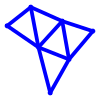
\includegraphics[width=1cm]{tinynet2} & $\times$ 100 &
      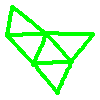
\includegraphics[width=1cm]{tinynet3} & $\times$ 100
    \end{tabular}
  };

  \node (rect3) [below=of rect2, box] { };
  \node at (rect3.north) [anchor=north] {\uline{300 epidemics}};
  \node (b) [above=4pt of rect3.south] {
    \begin{tabular}{m{0.5cm} m{1cm} m{0.5cm} m{1cm} m{0.5cm} m{1cm}}
      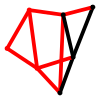
\includegraphics[width=1cm]{tinyepi1} & $\times$ 100 &
      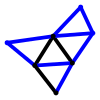
\includegraphics[width=1cm]{tinyepi2} & $\times$ 100 &
      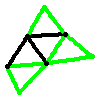
\includegraphics[width=1cm]{tinyepi3} & $\times$ 100
    \end{tabular}
  };

  \node (rect4) [below=of rect3, box] { };
  \node at (rect4.north) [anchor=north] {\uline{300 transmission trees}};
  \node (b) [above=4pt of rect4.south] {
    \begin{tabular}{m{0.5cm} m{1cm} m{0.5cm} m{1cm} m{0.5cm} m{1cm}}
      
\includegraphics[width=1cm]{tinytree1} & $\times$ 100 &
      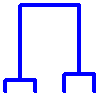
\includegraphics[width=1cm]{tinytree2} & $\times$ 100 &
      
\includegraphics[width=1cm]{tinytree3} & $\times$ 100
    \end{tabular}
  };

  \node (rect5) [right=of rect1, box] { };
  \node at (rect5.north) [anchor=north, text width=\boxw, align=center] {
    \uline{42 kernel matrices ($300 \times 300$)} \\ \vspace{4pt}
    $\lambda$ = \{ \nicefrac18, \nicefrac14, \nicefrac12, 1, 2, 4, 8 \} \\
    $\sigma$ = \{ 0.2, 0.3, 0.4 \} \\
    nLTT = \{ yes, no \} \\
  };

  \node (rect6) [below=of rect5, box] { };
  \node at (rect6.north) [anchor=north, text width=\boxw, align=center] {
    \uline{42 cross validations} \\ \hfill \\
    R$^2$ $\times$ 42
  };

  \node (rect7) [below=of rect6, box] { };
  \node at (rect7.north) [anchor=north, text width=\boxw, align=center] {
    \uline{optimal kernel meta-parameters} \\ \hfill \\
    $\lambda$ = 4,\; $\sigma$ = 0.3,\; nLTT = no
  };

  \node (rect8) [below=of rect7, minimum width=\boxw, minimum height=\boxh,
                 align=center, text width=\boxw] {
    repeat 8 times \\
    \vspace{4pt}
    infected nodes = \{ 500, 1000, 2000 \} \\
    sampled nodes = \{ 100, 500, 1000 \}
  };

  \coordinate [left=0.5 of rect5.west] (r5w);
  \coordinate [below=0.5cm of r] (r1ssw);
  \coordinate [below=of r1ssw] (r2nnw);
  \coordinate [below=0.5cm of g] (r1sse);
  \coordinate [below=of r1sse] (r2nne);
  \coordinate [below=3.5cm of r] (r2ssw);
  \coordinate [below=3.5cm of g] (r2sse);
  \coordinate [below=4.5cm of r] (r3nnw);
  \coordinate [below=4.5cm of g] (r3nne);
  \coordinate [below=6.5cm of r] (r3ssw);
  \coordinate [below=6.5cm of g] (r3sse);
  \coordinate [below=7.5cm of r] (r4nnw);
  \coordinate [below=7.5cm of g] (r4nne);
  \coordinate [below=0.5cm of rect4.north east] (r4ene);
  \coordinate [above=0.5cm of rect4.south east] (r4ese);

  \draw[next] (r1ssw) -- (r2nnw);
  \draw[next] (r1ssw) -- ($(r2nnw) + (-0.5cm, 0cm)$);
  \draw[next] (r1ssw) -- ($(r2nnw) + (0.5cm, 0cm)$);
  \draw[next] (r1sse) -- (r2nne);
  \draw[next] (r1sse) -- ($(r2nne) + (-0.5cm, 0cm)$);
  \draw[next] (r1sse) -- ($(r2nne) + (0.5cm, 0cm)$);
  \draw[next] (rect1.south) -- (rect2.north);
  \draw[next] (rect1.south) -- ($(rect2.north) + (-0.5cm, 0cm)$);
  \draw[next] (rect1.south) -- ($(rect2.north) + (0.5cm, 0cm)$);
  \draw [next] (rect2) -- (rect3);
  \draw [next] (r2ssw) -- (r3nnw);
  \draw [next] (r2sse) -- (r3nne);
  \draw [next] (rect3) -- (rect4);
  \draw [next] (r3ssw) -- (r4nnw);
  \draw [next] (r3sse) -- (r4nne);
  \draw [next] (rect4.east) -| (r5w) -- (rect5);
  \draw [thick] (r4ene) -- ++ (0.5cm, -0.5cm);
  \draw [thick] (r4ese) -- ++ (0.5cm, 0.5cm);
  \draw [next] (rect5) -- (rect6);
  \draw [next] (rect6) -- (rect7);
\end{tikzpicture}

\end{document}

  \caption[Variables used in tree kernel simulation experiments]
  {
    Values of parameters and other variables used in tree kernel simulation
    experiments. Each row corresponds to one of the \gls{BA} model parameters.
    One kernel matrix was created for every combination of values except the
    one indicated in the ``varied parameter'' column, which was varied when
    producing simulated trees.
  }
  \label{tab:kernelexpt}
\end{table}

\begin{table}[ht]
  \centering
  \begin{tabular}{cccccccc}
  parameter & grid values & test values & $N$ & $\alpha$ & $m$ & $I$ & tips \\
  \hline
  $N$ & 1050, 1125, \ldots, 15000 & 1000, 3000, \ldots, 15000 & - & 1.0 & 2 & 1000 & 100, 500, 1000 \\
  $\alpha$ & 0, 0.01, \ldots, 2 & 0, 0.25, \ldots 2 & 5000 & - & 2 & 1000 & 100, 500, 1000 \\
  $m$ & 1, 2, \ldots, 6 & 1, 2, \ldots 6 & 5000 & 1.0 & - & 1000 & 100, 500, 1000 \\
  $I$ & 500, 525, \ldots, 5000 & 500, 1000, 1500, 2000 & 5000 & 1.0 & 2 & - & 100, 500 \\
  \hline
\end{tabular}

  \caption[Variables used in grid search experiments]
  {
    Variables and \gls{BA} parameter values used for grid search experiments. 
    Trees were simulated under the test values, and compared to a grid of trees
    simulated under the grid values. Kernel scores were used to calculate point
    estimates and credible intervals for the test values.
  }
  \label{tab:gridexpt}
\end{table}
\end{landscape}

\begin{figure}[ht]
  \centering
  \includegraphics{kernel-expt.pdf}
  \caption[Schematic of experiments investigating impact of BA model parameters
           on tree shape.]{
    Schematic of experiments designed to investigate the impact of variations
    in BA model parameters on transmission tree shapes. The parameters of the
    BA model were varied one at a time. Transmission trees were simulated under
    three different values of each parameter, then compared pairwise using the
    tree kernel. Classifiers were constructed for each parameter, and their
    accuracy was evaluated by cross-validation. Kernel-PCA projections were
    used to visually examine the separation of the trees in the feature space
    defined by the tree kernel.
  }
  \label{fig:kernelexpt}
\end{figure}

\subsubsection*{Grid search}

As in the previous section, we will begin by describing a single experiment,
and then list the variables for which similar experiments were performed. We
varied \gls{alpha} along a narrowly spaced grid of values: 0, 0.01, \ldots, 2.
For each value, fifteen networks were generated with \software{igraph}, and
transmission trees were simulated over each using \software{nettree}. These
trees will be referred to as ``grid trees''. Next, one further test tree was
simulated with the test value \gls{alpha} = 0. Both the grid trees and the test
tree had 500 tips, and were simulated with the other \gls{BA} parameters set to
$N$ = 5000, $m$ = 2, and $I$ = 1000. The test tree was compared to each of the
grid trees using the tree kernel, with the meta-parameters set to $\lambda =
0.3$ and $\sigma = 4$, using the \software{treekernel} binary. The median
kernel score was calculated for each grid value, and the scores were normalized
such that the area under the curve was equal to 1. The grid value with the
highest median kernel score was taken as the point estimate for the test value,
and a 95\% credible interval was obtained using the \software{hpd} function in
the \software{TeachingDemos} package~\autocite{snow2013teachingdemos}.

Each experiment of the type just described was repeated ten times with the same
test value. Similar experiments were performed for each of the four \gls{BA}
parameters, with several test values and trees of varying sizes. The variables
are listed in \cref{tab:gridexpt}. A graphical schematic of the grid search
experiments is shown in \cref{fig:gridexpt}. 
%Spearman's correlation was used to test whether the number of tips in the tree
%was correlated with the acccuracy of the point estimates. One-way \gls{ANOVA}
%was used to test whether the accuracy of the point estimates were significantly
%higher for any parameter values. If so, the distribution of errors was examined
%to choose a suitable post hoc test. If there appeared to be a correlation
%between the parameter value and the accuracy of the estimate, Spearman's
%correlation was calculated. If there were one or more particular values which
%appeared to have lower error, we used the Wilcoxon rank-sum test.

\begin{figure}[ht]
  \centering
  \includegraphics[width=\textwidth]{gridsearch-expt}
  \caption[Schematic of grid search experiment.]{
    Graphical schematic of grid search experiments used to investigate \gls{BA}
    model parameters. Trees were simulated along a narrowly spaced grid of
    parameter values (``grid trees''). Separate trees were simulated for a
    small subset of the grid values (``test trees''). Each test tree was
    compared to every grid tree using the tree kernel, and the resulting kernel
    scores were normalized to resemble a probability density from which the
    mode and 95\% highest density interval were calculated.
  }
  \label{fig:gridexpt}
\end{figure}

\subsubsection*{Approximate Bayesian computation}

To test the full kernel-assisted \gls{ABC} algorithm, we simulated three trees each under
a variety of parameter values, and ran the \software{netabc} program to
estimate posterior distributions for the parameters. The parameter values and
priors used are listed in \cref{tab:abcexpt}. The tree kernel meta-parameters
were set to $\lambda = 0.3$ and $\sigma = 4$. The \gls{SMC} algorithm was run
with 1000 particles, five sampled datasets per particle, and the $\alpha$
parameter (not to be confused with the \gls{BA} preferential attachment
parameter, see \cref{subsubsec:adaptsmc}) set to 0.95. The algorithm was
stopped when the acceptance rate of the \gls{MH} kernel dropped below 1.5\%,
the same criterion used by \citeauthor{del2012adaptive}. Approximate marginal
posterior densities for each parameter were calculated using the
\software{density} function in \software{R} applied to the final weighted
population of particles. Credible intervals were obtained for each parameter
using the \software{HPDinterval} function in the \software{coda}
package~\autocite{plummer2006coda}.

\begin{table}[ht]
  \centering
  \begin{tabular}{ccc}
  parameter or variable & test values & prior \\
  \hline
  $N$ & 5000 & Uniform(500, 15000) \\
  $\alpha$ & 0, 0.5, 1, 1.5, 2 & Uniform(0, 2) \\
  $m$ & 2, 3, 4 & Uniform(1, 5) \\
  $I$ & 1000, 2000 & Uniform (1000, 2000) \\
  tips & 500 & - \\
  \hline
\end{tabular}

  \caption[Variables used in grid search experiments]
  {
    Variables and \gls{BA} parameter values used for \gls{ABC} validation
    experiments. Trees were simulated under the test values, and
    kernel-assisted \gls{ABC} was used to re-estimate posterior distributions for the
    \gls{BA} parameters without training.
  }
  \label{tab:abcexpt}
\end{table}

%\subsubsection*{Characterization of power-law exponent in Barab\'asi-Albert networks}
%
%Most studies of social network or transmission network
%parameters~\autocite[e.g.][]{liljeros2001web, jones2003assessment,
%schneeberger2004scale, brown2011transmission} report the coefficient
%\gls{gamma} of the power law degree distribution. To make our results
%comparable to previous work, we used simulated networks to investigate the
%relationship between the \gls{BA} model parameters and \gls{gamma}. A network
%was simulated for each combination of parameters listed in
%\cref{tab:gammaexpt}. A power law distribution was fitted to the degree
%distribution of each simulated network using the \software{fit\_power\_law}
%function in \software{igraph} with the `R.mle' implementation. We fitted a
%\gls{GLM} with Gamma-distributed errors and a log link function to the observed
%distribution of \gls{gamma} values, with \gls{alpha}, \gls{m}, \gls{N}, and all
%possible interaction terms as predictors.
%
%\begin{table}
%  \centering
%  \begin{tabular}{cc}
  parameter & values \\
  \hline
  $N$ & 500, 600, \ldots, 15000 \\
  $\alpha$ & 0, 0.01, \ldots, 2 \\
  $m$ & 1, 2, \ldots, 8 \\
  \hline
\end{tabular}

%  \caption[\gls{BA} parameters used as input \gls{GLM} predicting $\gamma$]
%  {
%    \gls{BA} model parameters used as input to \gls{GLM} predicting power law
%    exponent $\gamma$. One network was simulated with each combination of
%    parameters, and $\gamma$ was calculated for each network. A \gls{GLM} with
%    Gamma-distributed errors and a log link function was fit to the $\gamma$
%    values with all parameters and interaction terms as predictors.
%  }
%  \label{tab:gammaexpt}
%\end{table}

%To evaluate the effects of the true parameter values on the accuracy of the
%\gls{MAP} estimates, we analysed each parameter individually using a \gls{GLM}
%(four \glspl{GLM} total). The response variable was the error of the point
%estimate, and the predictor variables were the true values of \gls{alpha},
%\gls{I}, and \gls{m}. We did not test for differences across true values of
%\gls{N}, because \gls{N} was not varied in these simulations. The distribution
%family and link function for each \gls{GLM} were chosen by examination of
%residual plots and \gls{AIC} of the model fits. For \gls{alpha}, \gls{I}, and
%\gls{N}, we used the Gamma distribution with the inverse link function. For
%\gls{m}, we used the Poisson distribution with the log link function. To
%allow for the possibility that the relationships between parameters and error
%rates were nonlinear, the true parameter values were treated as discrete rather
%than continuous predictors. When significant associations were found by the
%\glspl{GLM}, additional post hoc tests were performed based on the observed
%relationship between the error rate and true parameter value in question. If
%the relationship appeared to be monotonic, Spearman's correlation was
%calculated. Otherwise, if there were particular values which appeared to have a
%higher error rate than the others, the Wilcoxon rank-sum test was used to check
%for a significant difference between the two groups.

Two further experiments were performed to address potential sources of error.
To evaluate the effect of model misspecification in the case of heterogeneity
among nodes, we generated a network where half the nodes were attached with
power $\alpha$ = 0.5, and the other half with power $\alpha$ = 1.5. The other
parameters for this network were $N$ = 5000, $I$ = 1000, and $m$ = 2. To
investigate the effects of potential sampling
bias~\autocite{karcher2016quantifying}, we simulated a transmission tree where
the tips were sampled in a peer-driven fashion, rather than at random. That is,
the probability to sample a node was twice as high if any of that node's
network peers had already been sampled. The parameters of this network were $N$
= 5000, $I$ = 2000, $m$ = 2, and $\alpha$ = 0.5.

\subsection{Application to HIV data}

Because the \gls{BA} model assumes a single connected contact network, it is
most appropriate to apply to groups of individuals who are epidemiologically
related. Therefore, we searched for published \gls{HIV} datasets which
originated from existing clusters, either phylogenetically or geographically
defined. In addition, we analysed an in-house dataset sampled from
\gls{HIV}-positive individuals in British Columbia, Canada (the ``BC data'').
The datasets are summarized in \cref{tab:data}.

\begin{table}[ht]
  \centering
  \begin{tabular}{ccccc}
  Reference & Sequences ($n$) & Location & Risk group & Gene \\
  \hline
  \textcite{wang2015targeting} & 173 & Beijing, China & MSM & \textit{pol} \\
  \textcite{cuevas2009hiv} & 287 & Basque Country, Spain & mixed & \textit{pol} \\
  \textcite{novitsky2013phylogenetic} & \multirow{2}{*}{180} &
  \multirow{2}{*}{Mochudi, Botswana} & \multirow{2}{*}{HET} &
  \multirow{2}{*}{\textit{env}} \\ \textcite{novitsky2014impact} \\
  \textcite{li2015hiv} & 280 & Shanghai, China & MSM & \textit{pol} \\
  \textcite{niculescu2015recent} & 136 & Romania & IDU & \textit{pol} \\
  unpublished & 399 & British Columbia, Canada & IDU & \textit{pol} \\
  \hline
\end{tabular}

  \caption[Characteristics of published HIV datasets analyzed with \software{netabc}.]
  {
    Characteristics of published HIV datasets analyzed with \software{netabc}. 
    Abbreviations: MSM, men who have sex with men; HET, heterosexual; IDU,
    injection drug users. The \textcite{novitsky2013phylogenetic,novitsky2014impact} data
    were sampled from a primarily heterosexual risk environment, but did not
    explicitly exclude other risk factors.
  }
  \label{tab:data}
\end{table}

We downloaded all sequences associated with each published study from GenBank.
For the \textcite{novitsky2014impact} data, each \textit{env} sequence was
aligned pairwise to the HXB2 reference sequence (GenBank accession number
K03455) and the hypervariable regions were clipped out with
\software{BioPython} version 1.66+~\autocite{cock2009biopython}. Sequences were
multiply aligned using \software{MUSCLE} version 3.8.31
\autocite{edgar2004muscle}, and alignments were manually inspected with
\software{Seaview} version 4.4.2 \autocite{gouy2010seaview}. Phylogenies were
constructed from the nucleotide alignments by approximate maximum likelihood
using \software{FastTree2} version 2.1.7 \autocite{price2010fasttree} with the
\gls{GTR} model~\autocite{tavare1986some}. Transmission trees were estimated by
rooting and time-scaling the phylogenies by root-to-tip regression, using a
modified version of Path-O-Gen (distributed as part of
BEAST~\autocite{drummond2007beast}) as described
previously~\autocite{poon2015phylodynamic}. 

Three of the datasets \autocite[][and the BC data]{li2015hiv,novitsky2014impact}
were initially much larger than the others, containing 1265, 1299, and 7923
sequences respectively. To ensure that the analyses were comparable, we reduced
these to a number of sequences similar to the smaller datasets. For the
\citeauthor{li2015hiv} and BC datasets, we detected clusters of size 280 and
399 respectively using a patristic distance cutoff of 0.02 as described
previously~\autocite{poon2015impact}. Only sequences within these clusters were
carried forward. For the \textcite{novitsky2014impact} data, no large clusters
were detected using the same cutoff, so we analysed a subtree of size 180
chosen arbitrarily.

Empirical studies of contact networks often report the exponent $\gamma$ of the
power law degree distribution. To compare our results to the literature, we
simulated 100 networks each according to the \gls{MAP} parameter estimates
obtained for each investigated dataset. The power-law exponent $\gamma$ was
calculated for each network using the \software{fit\_power\_law} function in
\software{igraph}, with the `R.mle' implementation. The median of the 100
$\gamma$ values was taken as a point estimate for the associated dataset.

For all datasets, we used the priors $\alpha$ $\sim$ Uniform(0, 2) and $N$ and
$I$ jointly uniform on the region \{$n \leq N \leq 10000$, $n \leq I \leq
10000$, $I \leq N$\}, where $n$ is the number of tips in the tree (see
\cref{tab:data}). Since the value $m = 1$ produces networks with no cycles,
which we considered fairly implausible, we ran one analysis with the prior $m
\sim$ DiscreteUniform(1, 5), and one with the prior $m \sim$ DiscreteUniform(2,
5). The other parameters to the SMC algorithm were the same as used for the
simulation experiments, except that we used 10000 particles instead of 1000 to
increase the accuracy of the estimated posterior. This was computationally
feasible due to the small number of runs required for this analysis.
